% !TEX root = ../../fyp.tex
\documentclass[../../fyp.tex]{subfiles}

\begin{document} 
In pursuit of the objectives laid out in chapter \ref{chap:introduction} we develop a framework that is centered around TSA. Limiting the scope of the framework to the field of TSA allows us to extrapolate the time-consuming processing that typically comprise an experiment, and provide an API which exposes this functionality to any TSA model built using the framework, reducing the time required to implement and evaluate each model. Moreover, this approach isolates the evaluation environment from the model, making it consistent across experiments using different model implementations.

To account for numerous forms that TSA model approached can adopt, user-extensibility is an essential component of the API design, providing a means of adding functionality at both the data preparation and model evaluation stages. 

Finally, it is imperative that a clear delineation is made between aspects of the framework with which the user may interface, and other internal elements which should be abstracted from the end-user, which facilitates experimentation by making the framework more intuitive to use and reduces the risk of costly run-time errors.  

This chapter details the two primary modules of the framework, following each seminal component through the experiment pipeline and the respective design choices made in accordance with the aforementioned principles.

\begin{figure}[!ht]
	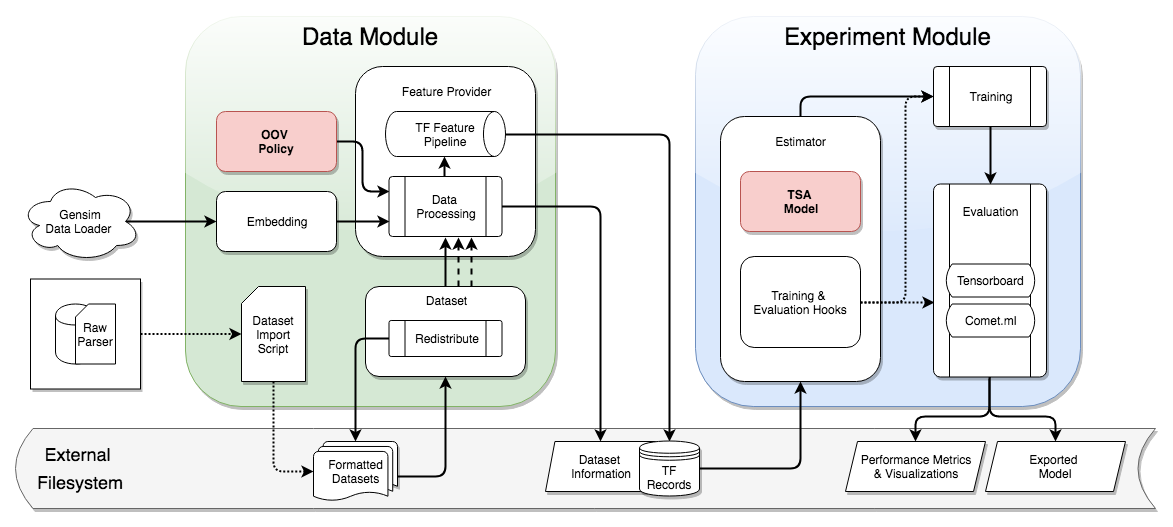
\includegraphics[width=\textwidth]{framework_block_diagram.png}
	\caption{Block diagram illustrating the separate modules, their constituent components and how these interact and communicate with each other.}
	\label{fig:framework_block_diagram}
\end{figure}

\section{Data Module} \label{sec:data_module}
\subfile{chapters/3-Design/3.1-DataModule}

\section{Experiment Module} \label{sec:experiment_module}
\subfile{chapters/3-Design/3.2-ExperimentModule}

\section{Summary}
We have discussed the design principles that were considered at each sub-component on a conceptual level, to address the objectives described in \S\ref{sec:objectives}. 

Furthermore, we have presented how each of these sub-components assemble to establish a framework which simplifies the process of implementing new TSA models and provides a static evaluation environment with robust metrics and informative visualizations. Chapter \ref{chap:implementation} shall expound on how the design principles outlined herein were actualized into code at particular stages of the framework.

\end{document}